\documentclass{article}
\usepackage{graphicx} % Required for inserting images
\usepackage{wrapfig}
\usepackage{hyperref}
\usepackage[export]{adjustbox}
\usepackage{geometry}
\geometry{a4paper,
 total={170mm,257mm},
 left=5mm,
 top=20mm}

\title{Gruppo B (Federico, Antonio, Pier, Angelo)}
\author{Giovanni Cisternini}
\date{December 2023}

\begin{document}
\tableofcontents

\maketitle


\section{Trama}
\subsection{Nemici}
\begin{table}
    \centering
    \begin{tabular}{|cr cr cr|}
        \hypertarget{doberman}{Doberman} & Mago & \hypertarget{granchio}{Granchio Gigante} \\
        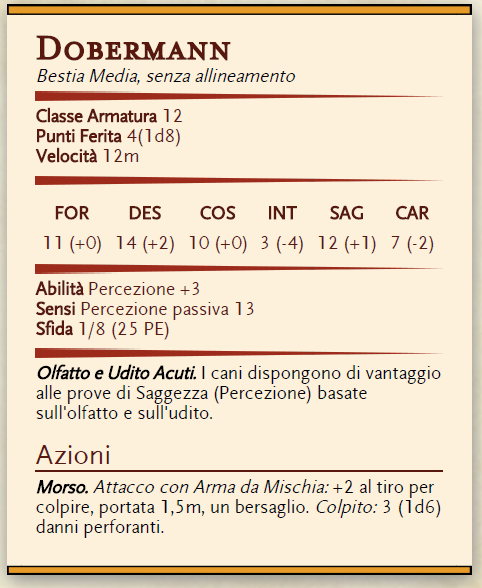
\includegraphics[width=4cm, height = 6 cm]{../Mostri/Doberman.png} &  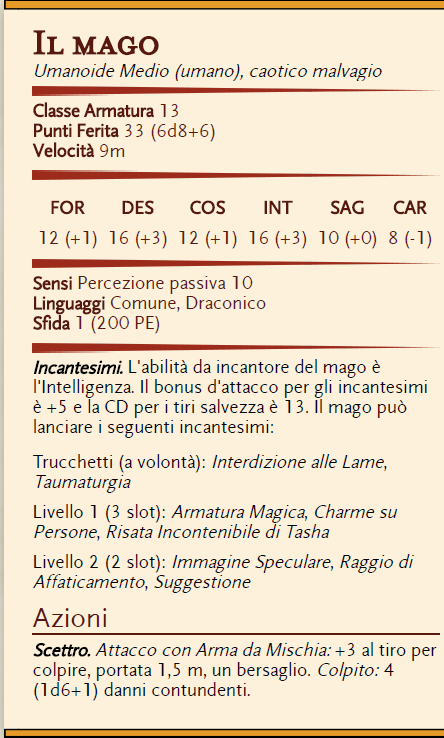
\includegraphics[width=4cm, height = 6 cm]{../Mostri/mago.png} &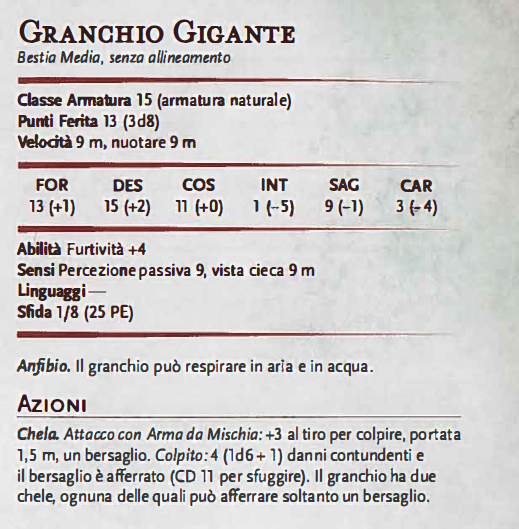
\includegraphics[width=4cm, height = 6 cm]{../Mostri/Granchio Gigante.PNG}
        \\
        \hypertarget{uomorana}{Uomorana} & Salamandra & \hypertarget{re}{ReDeiRospi}\\
        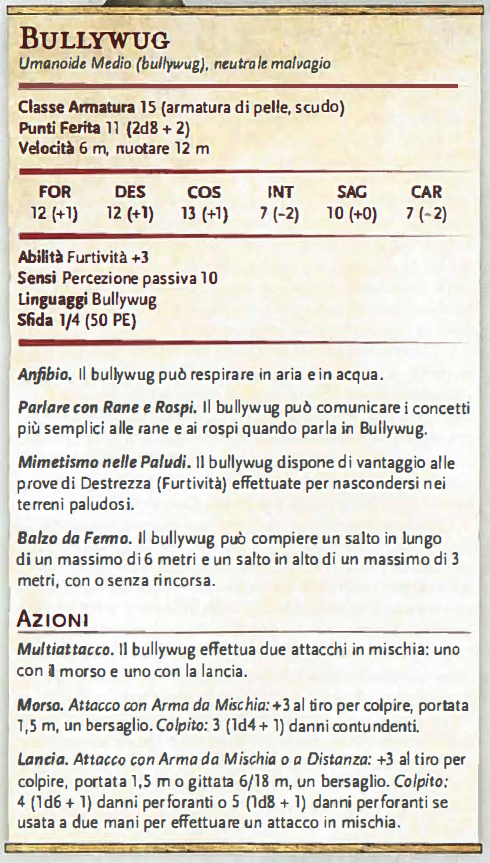
\includegraphics[width=4cm, height = 6 cm]{../Mostri/Bullywug.PNG} &  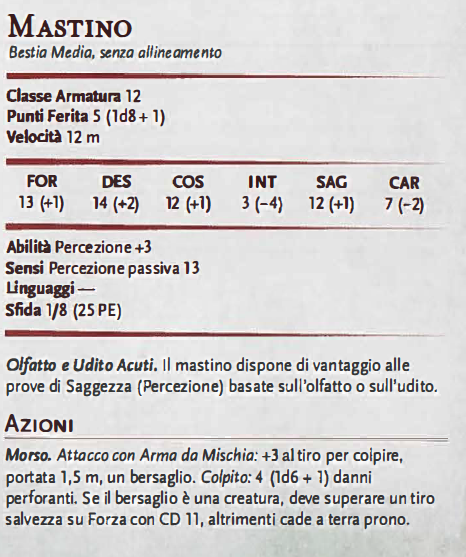
\includegraphics[width=4cm, height = 6 cm]{../Mostri/Mastino.PNG}&
        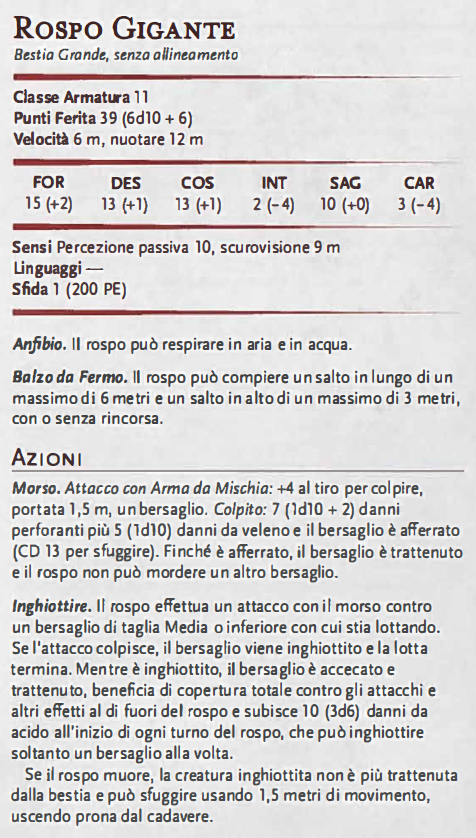
\includegraphics[width=4cm, height = 6 cm]{../Mostri/ReDeiRospi.PNG}\\
        \hypertarget{sciame}{Sciame Di Quipper} & \hypertarget{orco}{Orco} &  \hypertarget{bandito}{Bandito} \\
        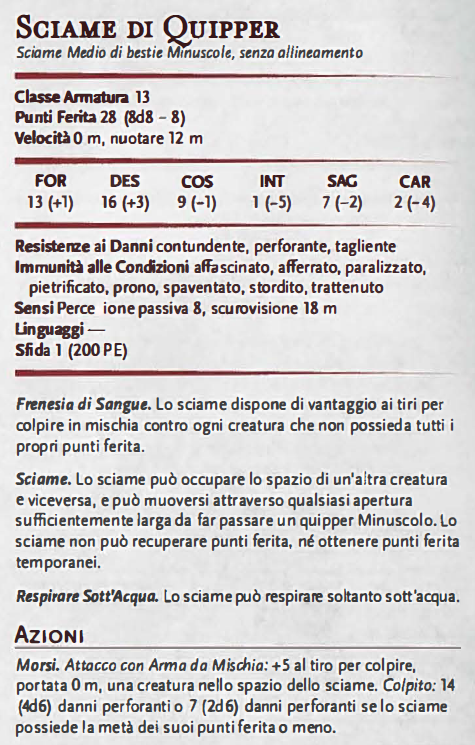
\includegraphics[width=4cm, height = 6 cm]{../Mostri/Sciame di Quippers.PNG} &  
        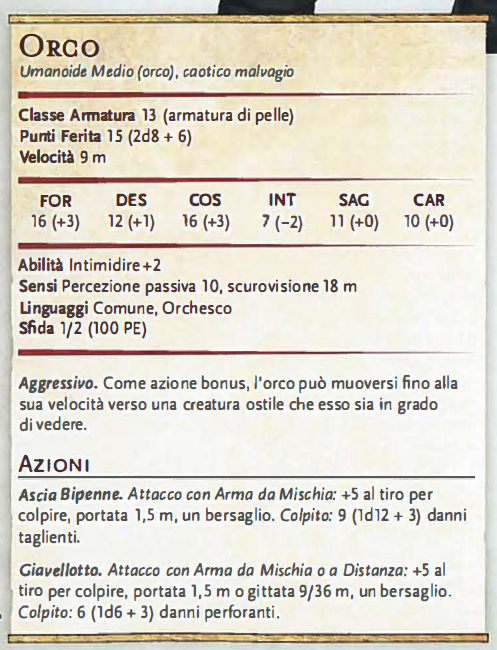
\includegraphics[width=4cm, height = 6 cm]{../Mostri/Orco.PNG} & 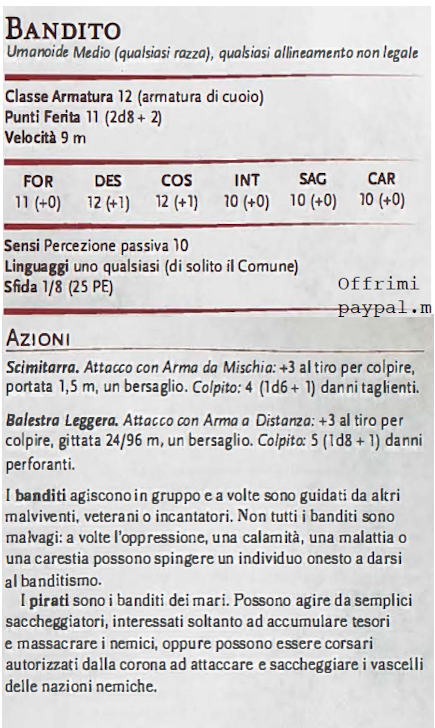
\includegraphics[width=4cm, height = 6 cm]{../Mostri/Bandito.PNG} \\ 
        \hypertarget{kenk}{Kenku} & \\
        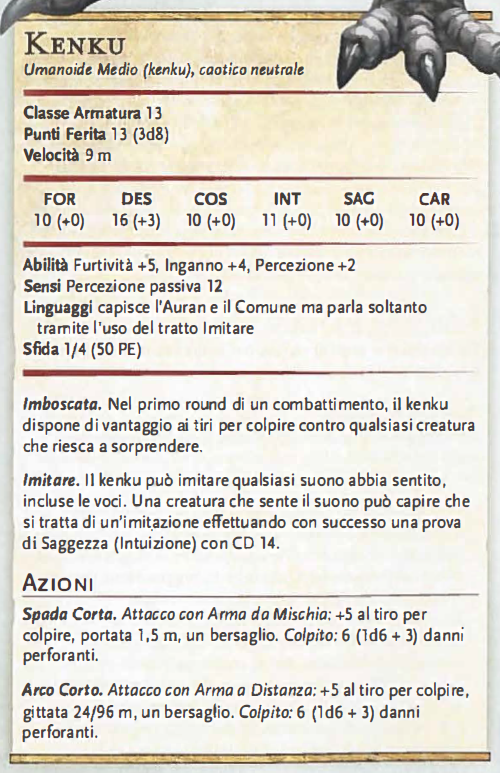
\includegraphics[width=4cm, height = 6 cm]{../Mostri/Kenku.PNG}

    \end{tabular}
 

\end{table}







\newpage
\subsection{La Torre del Mago (da Liv 1 a liv 2)}
\subsubsection{Sotterranei}
Scendendo, i personaggi arrivano in un corridoio costruito in pietra. Alcune torce emanano una luce tenue. Coloro che hanno Scurovisione riescono a vedere come se il luogo fosse illuminato. Gli altri hanno difficoltà a vedere come il corridoio prosegua. Il DM chiede ai giocatori di effettuare una prova di Saggezza (Percezione) con una Classe Difficoltà (CD) di 10. I personaggi senza Scurovisione hanno svantaggio. Con un successo sulla prova, i personaggi vedranno che, sul muro, dopo 9 metri, c'è una leva al posto di una torcia.Quando viene tirata la leva, si apre un passaggio segreto nel muro. Il passaggio conduce al dungeon che si trova nei sotterranei della torre (mostrato nella pianta qui a fianco). I numeri nella piatina corrispondono alla seguente lista dei luoghi. I quadrati nella mappa hanno un lato di 1,5 metri.
\begin{enumerate}
    \item \textbf{Ingresso} Entrando in questa stanza, i personaggi sentiranno il passaggio segreto che si richiude alle loro spalle. Sono prigionieri nel dungeon. Una voce echeggia nella stanza: \textit{Benvenuti nella mia torre amici. Sono così felice di avere finalmente degli ospiti per provare la mia splendida creazione.
Mi domando solo quanto a lungo sopravviverete.} \textsc{Questa prima stanza è grande e vuota. Il pavimento è bagnato e potete sentire l'eco del rumore di gocce d'acqua che cadono. Alcune torce illuminano questo luogo. Potete distinguere due porte sulla parete nord.}
    \item \textbf{Fossa} Anche questa stanza è vuota ma al centro c'è una trappola:
        \begin{itemize}
            \item Tiro su \textsc{Indagare}per scoprire la trappola CD 12
            \item TS Destrezza se ci cade CD 10
        \end{itemize}
    \item \textbf{Corridoio} \textsc{Entrando nel corridoio vedete quattro statue lungo i muri. Tra le statue ci sono delle torce appese e alcune porte. Potete sentire un movimento d'aria che suggerisce la presenza di un'apertura nella direzione della fine del corridoio.}
    \item \textbf{Trappola Velenosa} Aprire la porta equivale a far scattare la trappola (un ago sparato dal muro che attraversa la stanza e colpisce chi ha aperto la porta
        \begin{itemize}
            \item Tiro per colpire Trappola : d20 + 4
            \item TS Costituzione per non essere Avvelenato(svantaggio ai tiri per colpire e alle prove abilita finché non beve l'antidoto) CD 10
            \item \textsc{Indagare} sulla porta CD 15 trova la trappola
            \item \textsc{Rapidita di Mano} per disinnescare la trappola CD 18
            \item se entrando trovano uno scheletro con vestiti e borsa, nella borsa una pozione curativa (2d4+2)
        \end{itemize}
    \item \textbf{Canile} Ci sono 2 cani rabbiosi appena entrano combattimento con Doberman \newline
         ci sono poi, sulla parete opposta alla porta 5 gabbie, della quale 2 vuote in alto, in basso negli angoli ci sono 2 gabbie dalla quale sporgono degli stivali (Penelope e PG Pier) 
        CD per Aprire le Gabbie 12, CA lucchetto 19 PF 2
       
    \item \textbf{Scale} \textit{Sono così felice che siate sopravvissuti al mio dungeon.
Adesso, potrete affrontare le altre prove che ho preparato per voi. Vediamo se riposerete al primo piano per l'eternità!}

\end{enumerate}
\newpage
\subsubsection{Primo Piano}
    \textsc{Salendo le scale arrivate in una stanza ottagonale illuminata dalla grande vetrata che vedete di fronte a voi. I vetri colorati mostrano la figura di un drago.Sul pavimento c'è una grande cornice, delle stesse dimensioni della vetrata, e vari pezzi di legno di diverse forme.}
\subsubsection{Secondo Piano}
\textsc{Due grosse lucertole, in piedi sugli arti posteriori, vi aspettano.
Una è robusta e ben equipaggiata, sta in mezzo alla stanza.
L'altra è più esile e mantiene la distanza. "Benvenuti al piano
della morte" sibila il secondo lucertoloide mentre incocca una
freccia nel suo arco.}

\begin{enumerate}
    \item Shkiss ha una pozione antidoto
    \item Sgrolt ha una pozione curativa (2d4+2) 
\end{enumerate}

\subsubsection{Terzo Piano}
un'Altra stanza ottagonale... una stanza molto disordinata piena di scatole e barili. Nella parete opposta all'entrata c'è una porta. quando si avvicinano, si accorgono che è chiusa da 4 serrature. 
\begin{enumerate}
    \item Percezione CD 12, Una chiave si trova appesa al soffitto, ad una altezza di 3 metri. Si puo raggiungere scalando la parete con Atletica CD 15 (se cade 1d6 di danni), Se provano a tagliare la corda lanciando qualcosa CD 20 1 PF
    (si abbassa se si avvicinano)
    \item 2 piccoli forzieri : 1 pozione curativa, 1 la chiava. Forzieri con 20 PF. CD 12 Rapidita di mano per aprire.
    \item Chiave in un blocco di ghiaccio, ci impiega 5 ore a sciogliersi, con una fiamma si scioglie in pochi minuti. 
    \item L'ultima chiave si trova in una scatola in legno con una facciata di vetro, da cui si vede la struttura di un labirinto e attaccata alla scatola c'è una catenella con un magnete, e sul fianco della scatola c'è un buco da cui far uscire la chiave. Distruggere la scatola con 20 PF.
    \end{enumerate}

    dietro la porta c`è la scala che porta all'ultimo piano.
\subsubsection{Ultimo Piano}
\textsc{Miei cari ospiti, non mi aspettavo che sareste arrivati fino
all'ultimo piano della mia torre. Sono incantato di conoscervi
personalmente. Oggi è davvero un giorno speciale, ho avuto
l'opportunità di vedervi soffrire affrontando le mie prove e
avrò l'onore di porre fine alle vostre vite.}
Gli avventurieri
potrebbero provare a parlare col mago. Lui risponderà
ridendo e, se gli verranno chieste spiegazioni sul suo
comportamento, risponderà soltanto dicendo che si sta
divertendo.
Il mago non può lanciare incantesimi che danneggiano gli
avventurieri, ma userà la sua magia per impedire ai
personaggi di attaccare. Nel primo turno, usa Taumaturgia
nel tentativo di spaventare i personaggi.
Userà poi l'incantesimo Armatura Magica per aumentare la
propria CA oppure Immagine Speculare per schivare i colpi.
Successivamente lancia Interdizione alle Lame. Raggio di
Affaticamento previene i danni fisici, quindi il mago lo lancerà
contro Nadarr o Vidarr.
Risata Incontenibile di Tasha può essere usato per
bloccare Al . Charme su
Persone e Suggestione si rivelano utili per convincere a smettere di attaccare Si faccia attenzione alla durata degli incantesimi e alla
necessità di mantenere la concentrazione. Quando il mago
vuole danneggiare un personaggio, lo colpisce con lo scettro.
Il DM potrebbe evitare di farlo nei primi turni perché il mago
non ha molti punti ferita e, senza la protezione magica, non
riuscirebbe a sopravvivere a lungo.
Una volta sconfitto il mago, gli avventurieri sono
finalmente liberi. Nella stanza c'è una leva che apre il
passaggio segreto da cui i personaggi sono entrati nel
seminterrato. Troveranno inoltre 30 monete d'oro, gemme
per un valore di 20 monete d'oro e il libro degli incantesimi
del mago che contiene gli incantesimi usati dal mago stesso.

\subsection{il Re rospo} Nadar e Vidar vengono mandati vicino Neverwinter da Thorgrim, perché gli è arrivata una richiesta di aiuto da un suo vecchio conoscente (Fili-hip). Partono per un villaggio anonimo all'interno della foresta di Neverwinter. La richiesta è vaga, si parla di uomini rana , re rospi e rapimenti vari.  arrivano dal capo villaggio di nome Fili-hip, che spiega : gli uomini-rana hanno sempre vissuto pacificamente nella palude, ma di recente si sono fatti arroganti e aggressivi e hanno cominciato ad assalire la comunità alla luce del giorno. Di solito queste creature si accontentano di rubare una gallina o due, ma da un paio di mesi a questa parte hanno preso ad attaccare i viaggiatori per derubarli. Nelle ultime due settimane si sono spunti a rapite dei contadini: quattro persone sono già state trascinate nella palude!  i termini che impone sono troppo onerosi per i contadini: vuole 10 pezzi d’oro oppure 2 armi di metallo in buone condizioni per ogni persona che verrà riportata alla famiglia. Fornisce anche le indicazioni per raggiungere la palude. 
\subsubsection{Palude} Raggiunta la palude tiro su Sopravvivenza/Indagare CD 15 per trovare/notare le tracce di un uomo-rana e delle salamandre; se falliscono se lo trovano difronte dopo 200 metri, altrimenti riescono a seguirlo e tiro Furtivita per attacco a sorpresa. 
\begin{itemize}
    \item 1 \hyperlink{uomorana}{uomo rana}
    \item 2 salamandre giganti
    \item 4 \hyperlink{granchio}{granchi giganti}
\end{itemize}




Dopo questi scontri i personaggi: possono interrogare l’eventuale uomo-rana prigioniero per scoprire dove si trova la sua comunità, oppure possono cercare di seguire le tracce dei rapitori con una prova di Saggezza (Sopravvivenza) con Classe Difficoltà 12.
Se fallisce sbagliano strada e finiscono in uno stagno di alghe (Percezione CD 12 per accorgersene) dove trovano un banco di piccoli \hyperlink{sciame}{pesci carnivori}. Dopo aver ucciso i pesci, più in la vedono una casetta in paglia che poggia su un piccolo spiazzo di terra che sale sopra il livello della palude, se si avvicinano CD 14 Percezione passiva si accorgono di 2 paia di orme abbastanza grandi che escono dalla casa, se entrano e iniziano a rovistare :
\begin{itemize}
    \item In un bauletto aperto trovano 12 mr e una pozione guaritrice
    \item In un bauletto chiuso a chiave CD 13 Rapidita di mano, trovano 65 ma
\end{itemize}
\begin{itemize}
    \item se decidono di fare un riposo lungo chi deve salire al livello 2 e verso mezza notte si trovano 2 orchi che entrano in casa
    \item il più grosso ha addosso 12 mo e il più piccolo 18 di argento
\end{itemize}
Se non fallisce arrivano al villaggio degli uomini rana. Se decidono di riposare brevemente chi ha superato i 295-300 xp sale a livello 2 altrimenti usa il dado vita se vuole recuperare energie se fanno il riposo lungo tutti recuperano energia e chi ha superato gli XP sale a liv 2, ma durante la notte vengono attaccati da 2 orchi che si aggiravano nei dintorni.
La comunità degli uomini-rana è piuttosto selvaggia e spartana, non ci sono edifici veri e propri ma solo ripari di giunchi e qualche recinto dove vengono allevati granchi e gamberi di palude.
\subsubsection{Villaggio}
Nel villaggio si trovano quattro uomini-rana combattenti: tre assaltano i personaggi e uno resta a protezione del \hyperlink{re}{Re dei Rospi}. Gli altri umanoidi anfibi non hanno il coraggio per combattere e sebbene numerosi non affronteranno i personaggi. Il Re è un rospo della taglia di un orso bruno e dotato di una mente acuta come quella di un umano, e del dono della parola.
\subparagraph{Comportamento}
I mostri più animaleschi si comportano in base all’istinto, attaccando la preda più facile e che offre minor resistenza. Gli uomini-rana invece utilizzano rudimentali tattiche per fiancheggiare i nemici, coglierli di sorpresa e tenerli separati. Se vedono un incantatore in azione cercano di eliminarlo per primo. Si tengono lontani da avversari pesantemente corazzati.





\subsection{Waterdeep: il furto dei dragoni}
\subsubsection{Setting dell'avventura}
\subparagraph{Nemico principale: } Manshoon (Inverno)
\subparagraph{Interdizione Draconica di Ahghairon}: I dragonidi hanno incubi durante la notte. 
\begin{itemize}
    \item \textbf{Al}: Si sveglia fra le montagne del Quibaluk, riconosce la sua stanza all'interno del monastero, si guarda le mani [battito di palpebre] vede le sue mani infuocate [battito di palpebre] si ritrova seduto con davanti a lui una tazza di te un vecchietto che gli da le spalle e dice "Figliolo cosa volevi dirmi dunque ..." il vecchietto si gira lentamente, e la faccia inizia a cadere e prendere fuoco. Il vecchio ha un ghigno sul viso e nel mentre inizia a ridere, delle voci sussurrano "Assassino, Mostro, Demone", [battitto di palpebre] tutto quanto inizia a prendere fuoco e le sue mani sono nuovamente ricoperte di fuoco, tutto intorno al lui prende fuoco, prova ad alzarsi ma c'è il cadavere del suo maestro con tutta la pelle carbonizzata che con voce rauca "Mi vendicherò demone" ... Si sveglia.
    \item \textbf{Nadarr}: Apre gli occhi e si ritrova al timone della barca di pirati, il cielo è sereno ed è tutto tranquillo, il suo amico Vidar è li al suo fianco che sorride e beve con una bottiglia di rum in mano. [chiude le palpebre] Si ritrova nel mare in tempesta, prova a navigare la nave, ma viene sbalzata a destra e sinistra, cerca Vidar per chiedere aiuto, ma nessuno risponde. Si accorge che sulla nave non c'è nessuno. Lascia il timone e inizia a correre per la nave, guarda in cabina... nessuno ... guarda in stiva ... nessuno ... si avvicina alla polena e trova il suo amico Vidar legato e pieno di sangue... urla forte appena tenta di avvicinarsi ... cade in acqua e inizia ad affogare... si sveglia. 
\end{itemize}

\subsubsection{Il Viaggio}
\textbf{Distanza N-W}: 497 km (14 giorni) 

\paragraph{Mare dei Morti} (dopo 5 giorni di cammino) 
\textbf{Distanza per superare}: 4 giorni di cammino

\paragraph{	Descrizione } Dopo 5 giorni di cammino, iniziate a notare che il terreno inizia a diventare sempre umido, l'aria inizia a diventare più pesante e sentite sempre più bzz-bzz che tanto da fastidio nelle notti estive. All'orizzonte verso sud-ovest intravedete una lunga distesa d'acqua, e a sud- est una lunga distesa di colline. Man mano che vi avvicinate all'acqua, osservate che è sporca e putrida, e in lontananza, fra la nebbia che cala sull'acqua, notate alcuni relitti e isolette con alberi spogli in cima. Odorando  sentite puzza di stantio, ma la vostra strada verso waterdeep è li difronte a voi, solo un po' più umida e tetra a causa degli alberi. 

\paragraph{Incontri}
\subparagraph{Mephit del Fango}: Ogni tanto durante il loro percorso gli avventurieri scorgono al bordo della palude i mephit che si lamentano in continuazione in Aquan e Terran:  "Tesorooo, datemi i vostri tesori" "Sono cosi viscido e inutilee" "Ho tanta fameee".
\subparagraph{Coccodrillo}: Se provano ad immergersi, vengono attaccati da 1d4 di coccodrilli che potrebbero vedere con Percezione (16).
\subparagraph{Ragno Gigante}: Se nei pressi della curva decidono di entrare nella parte sinistra delle palude di 5-10 metri, fanno un tiro su percezione (12) e si accorgono nel ragno altrimenti si attaccano alla ragnatela (Forza 12 per staccarsi) e vengono attaccati da un 1 Ragno gigante. 
\subparagraph{Rudere e Vecchietto-Cannibale}: Verso la fine della palude c'è un vecchio rudere sulla parte sinistra del percorso, poco inoltrato e abbastanza visibile dalla strada. Mentre sono in carrozza vedono un vecchietto che sta arando il suo piccolo orticello, e mentre si avvicinano alza il capo e si avvicina alla strada e saluta con sorriso, cerca di convincerli a fermarsi per una tazza di te e per due chiacchiere perché vuole compagnia.  Ha sui 75 anni, si presenta come Jack. Jack è un vecchietto, di corporatura media, stempiato in testa ma con dei capelli grigi che formano un codino dietro la testa, due occhiali che scendono sul naso. Sembra una persona dai modi gentili, molto affabile ed invita i personaggi ad entrare e a prendere una tazza di te (una di queste è avvelenata con Torpore (Incapacitato per 18 ore) ). Jack tenta di tenere il più possibile i pg in casa e di non farli andare via, dicendo che li vuole suoi ospiti per mangiare tutti insieme e che se vogliono possono dormire li in casa, non ha molte brandine ma sicuramente un posto al caldo è meglio di uno fuori nella palude.
La casa di Jack, non è enorme, ma neanche piccolissima, dentro è si vecchia ma bene arredata, c'è un piccolo camino con dentro un pentolone da cui proviene un buon profumo, degli scaffali con spezie e cassetti con posate e coltelli, poi ci sono varie statuette in legno ovunque che rappresentano corpi di uomo e donna, sotto ogni statuetta c'è un nome . Se camminano per la casa , sotto un tappeto c'è una botola (Percezione 14), se chiedono cosa ci sia li sotto, si incupisce e dice "Non sono affari tuoi " in maniera rude, poi torno allegro " o meglio, nulla di interessante solo una piccolo ripostiglio con cianfrusaglie", dopo una mezz'ora il fuoco inizia a spegnersi e Jack si dilegua "Oh il fuoco si spegne, vado a fare altra legna", se uno di loro decide di accompagnarlo, accetta ben volentieri. Se fa domande insistenti Jack svia il discorso. Se si intrufolano nella botola, appena aprono sentono un tanfo incredibile e notano che sul coperchio della botola c'è del materiale resinoso che sembra serva per sigillare. Nella botola è buio, se non hanno scurovisione senza luce non vedono nulla, appena entrano vedono corpi appesi a dissanguarsi, un tavolo posto al centro con catene, attrezzi da macellaio appesi al muro e dei pezzi di carne sul bancone. Se entrano tutti, Jack li sorprende se nessuno ha perc. passiva di almeno 15, e li chiude dentro. Se invece resta qualcuno di guardia, se sono davanti la porta vedono Jack arrivare, altrimenti Jack si ferma poco prima e vede la botola aperta e scappa nella foresta per poi seguirli nella foresta una volta andati via.   
   

\subparagraph*{Statistiche Principali:}
\begin{itemize}
  \item \textbf{Forza:} 12 (+1)
  \item \textbf{Destrezza:} 16 (+3)
  \item \textbf{Costituzione:} 12 (+1)
  \item \textbf{Intelligenza:} 10 (+0)
  \item \textbf{Saggezza:} 10 (+0)
  \item \textbf{Carisma:} 14 (+2)
\end{itemize}

\subparagraph*{Punti Ferita (PF):}
60 (8d8 + 24)

\subparagraph*{Difesa:}
\begin{itemize}
  \item \textbf{Classe Armatura (CA):} 14
  \item \textbf{Iniziativa:} +3
\end{itemize}

\subparagraph*{Competenze:}
\begin{itemize}
  \item Abilità Acrobatica (+5)
  \item Furtività (+5)
  \item Inganno (+4)
  \item Investigare (+3)
\end{itemize}

\subparagraph*{Attacchi:}
\begin{itemize}
  \item \textbf{Dagger (Pugnale):} +5 al colpire, 1d4 + 3 danni perforanti
\end{itemize}

\subparagraph*{Abilità di Classe:}
\begin{itemize}
  \item \textbf{Insightful Fighting:} Può usare l'Intelligenza invece della Forza o Destrezza per le prove di caratteristica per le competenze di Ladro.
  \item \textbf{Sneak Attack:} Può infliggere 1d6 danni aggiuntivi quando effettua un attacco con vantaggio o quando un alleato si trova entro 5 piedi dal bersaglio.
  \item \textbf{Thieves' Cant:} Può comunicare segretamente con altri ladri usando un linguaggio segreto.
\end{itemize}

\subparagraph*{Abilità di Assassino:}
\begin{itemize}
  \item \textbf{Assassinate:} Ha vantaggio negli attacchi contro creature non consapevoli della sua presenza.
  \item \textbf{Occhi nelle Ombre:} Può vedere nella penombra e nell'oscurità con visione buia fino a 60 piedi.
\end{itemize}

\subparagraph*{Tattiche di Combattimento:}
Jack preferisce attaccare di nascosto, cercando di ottenere l'Iniziativa per attivare il suo Sneak Attack. Utilizzerà l'Insightful Fighting per sfruttare la sua intelligenza nelle prove di caratteristica, cercando di individuare debolezze nei suoi avversari. Può cercare di mimetizzarsi tra la folla o nelle ombre per sorprendere i suoi nemici.

\subparagraph{Monti della Spada: Valle}
A valle dei monti della spada, in mezzo ai boschi che li circondano c'è un piccolo gruppo di Gnoll, se i personaggi fanno troppo rumore attirano la loro attenzione, e durante la notte verranno attaccati da 1d6 di Gnoll. 

\subsubsection{Arrivo a Waterdeep : Capitolo 1}

\paragraph{Rissa in Teverna: Portale Spalancato}
\subparagraph{Descrizione}Siete seduti attorno a un solido tavolo di legno illuminato
dalla luce intensa di una candela e coperto di piatti
ormai svuotati e di boccali mezzi pieni. Il frastuono
dei giocatori d'azzardo che gridano e degli avventurieri
ubriachi che intonano canzoni sconce rischia di soffocare
la musica stonata di un giovane bardo che strimpella con
il suo liuto qualche tavolo più in là.
Poi un grido sovrasta tutti gli altri rumori: “Scrofa! Ti
piace uccidere i miei amici, eh?” Poi una mezzorca alta più
di due metri viene colpita da un violento pugno sferrato
da un umano la cui testa rasata è ricoperta di tatuaggi
a forma di occhio. Altri quattro umani si schierano alle
sue spalle, pronti a unirsi alla rissa. La mezzorca fa
scrocchiare le nocche delle mani, ruggisce e si avventa
sulla figura tatuata... ma prima di vedere se qualcuno
versa del sangue, un gruppo di avventori si ammassa
attorno ai lottatori e vi blocca la vista. Cosa fate?

\subparagraph{Rissa}I combattenti umani sono cinque membri della Gilda
di Xanathar (CM \hyperlink{banditi}{banditi} umani). Quello con gli occhi
tatuati sul cranio pelato è il loro capo, \hyperlink{krent}{ Krentz}. La loro
avversaria, \hyperlink{yagra}{Yagra Strongfist}, è una mezzorca al servizio Se
degli Zhentarim . Yagra combatte per una
questione d'orgoglio.

\begin{itemize}
    \item \textbf{Immischiarsi} Se i personaggi scelgono di unirsi alla mischia, il DM
chiede a tutti di tirare per l'iniziativa, ma lo scontro sarà
quasi finito quando riusciranno a farsi strada tra il pubblico
rumoreggiante. A Krentz rimangono soltanto 3 punti ferita
e cerca di sottrarsi alla presa di Yagra, ma gli altri quattro
membri della Gilda di Xanathar sono pronti ad avventarsi
su di lei.
Per staccare Yagra da Krentz è richiesta una prova
di Forza contesa con la prova di Forza di Yagra. Se i
personaggi la aiutano, Yagra li ringrazia, ma resta delusa
dal fatto che si siano immischiati nel combattimento.
Il DM dovrà ricordare in che modo i personaggi
interagiscono con Krentz in questa scena. Se l’uomo
sopravvive, i personaggi potrebbero incontrarlo di nuovo
in uno dei nascondigli fognari della Gilda di Xanathar (vedi
l’area Q5 a pagina 28).
\item \textbf{Tenersi Da Parte} Se i personaggi non interferiscono nella lotta, Yagra
tramortisce Krentz, ma poi i compagni dell’uomo la
malmenano fino a farla svenire. Durnan, il proprietario del
Portale Spalancato, indica loro la porta. “Fuori!” intima e i
membri della Gilda di Xanathar fuggono portandosi dietro
il corpo privo di sensi di Krentz.

\end{itemize}

\paragraph{UN TROLL E I SUOI AMICI}
Nel terzo round della rissa, entra in scena un nuovo
problema dal pozzo aperto che si trova al centro della sala
comune del Portale Spalancato:

\subparagraph{Descrizione}Alcune grida d'allarme annunciano l'improvvisa
apparizione di una creatura massiccia che emerge
dal condotto al centro della sala comune: un mostro
dalla pelle verde e bozzolosa, i capelli neri lunghi e
aggrovigliati, il naso adunco lungo quanto una carota
e occhi iniettati di sangue. Quando mostra le zanne
ingiallite e ulula, notate che una mezza dozzina di
creature simili a pipistrelli sono avvinghiate al suo corpo,
mentre altre tre gli volano intorno come mosche. Tutti
gli avventori della taverna reagiscono terrorizzati, ad dell'oste, Durnan, che grida “Troll".

\subparagraph{Cosa succe}
Il \hyperlink{troll}{ troll}, che attualmente possiede 44 punti ferita, è salito
fin qui arrampicandosi dal primo livello di Sottomonte per
cibarsi di un po' di saporita carne umanoide, portando nove
\hyperlink{uccelli}{uccelli stigei} con sé. Una volta giunto nella sala comune,
il troll si erge in tutta la sua altezza di 2,7 metri e tira per
l'iniziativa. Anche gli uccelli stigei tirano per l'iniziativa,
ma soltanto i tre che volano sopra il troll costituiscono una
minaccia. Gli altri hanno attinto abbondantemente al sangue
del troll e sono gonfi, quindi tornano in volo all’interno del
pozzo per digerire il pasto. Man mano che il troll rigenera,
gli effetti della perdita di sangue diventano meno evidenti.
La maggior parte degli avventori e del personale della
taverna fugge o cerca riparo non appena vede il troll. Gli
uccelli stigei attaccano i personaggi più vicini, mentre
\hyperlink{Duran}{Durnan} (vedi l'’appendice B) sfodera il suo spadone,
scavalca il bancone con un balzo e affronta il mostro in
persona. Mentre attacca, ordina ai personaggi di pensare
agli uccelli stigei, poi getta addosso al troll una fiasca d'olio
per lampade a cui appicca il fuoco. Se Yagra è ancora
cosciente, si unisce allo scontro. Se qualche personaggio
contribuisce a sconfiggere il troll, Durnan lo ringrazia con
modi spicci: “Hai combattuto bene.”
Se uno o più personaggi scendono a 0 punti ferita
durante lo scontro, i membri del personale del Portale
Spalancato intervengono per stabilizzarli.

\paragraph{Incontro con Volo} 
Una volta che il troll e gli uccelli stigei sono stati tolti di
mezzo, Volo si fa strada tra la massa di avventori che si
era allontanata dal mostro e si fa avanti per salutare i
personaggi, lodandoli sperticatamente per il loro coraggio
(che siano lodi meritate o meno): “Voi siete gli avventurieri mandati dal mio buon amico Thorgrim,
dico bene? Avrei bisogno del vostro aiuto. Troviamo un
tavolo per parlare, che ne dite?”
Volothamp Geddarm è noto alla cittadinanza di
Waterdeep per essere un fanfarone che tende ad abbellire
i fatti a suo piacimento. Nonostante i suoi difetti, Volo
è però un individuo dal cuore tenero che tiene molto ai
suoi amici e attualmente è preoccupato per la sorte di
uno di loro. Inizialmente presenta la sua richiesta con un
atteggiamento suadente e misterioso, ma presto le sue
parole tradiscono un’accorata preoccupazione.

\subparagraph{Descrizione} La figura che vi ha contattato si accarezza i baffi, si
aggiusta il cappello spiovente e si stringe la sciarpa
al collo. “Volothamp Geddarm, cronachista, mago e
celebrità, al vostro servizio. Immagino abbiate notato che
in queste ultime decadi la città si è fatta violenta. Non
vedevo tanti spargimenti di sangue dalla mia ultima visita
a Baldur's Gate! Ma ora temo di avere involontariamente
coinvolto un amico in questi odiosi fatti di violenza.”
“Il mio amico si chiama Floon Blagmaar. Ha più
bellezza che cervello e ho paura che un paio di notti fa
abbia sbagliato strada mentre tornava a casa e sia stato
rapito... o peggio. Se accettate di rintracciarlo per me al
più presto, vi posso offrire dieci dragoni a testa ora, e
dieci volte tanto quando troverete Floon. Posso contare
su voi nell'ora del bisogno?”

\subparagraph{Cosa succede} Volo consegna a ogni personaggio un piccolo borsello
contenente 10 mo semplicemente per avere accettato
la sua missione. Se un personaggio vuole scoprire le
sue intenzioni, deve effettuare una prova di Saggezza
(Intuizione) con CD 10. In caso di successo, capisce che
Volo è onesto, ma forse sta esagerando un po' riguardo
all'entità della ricompensa (Volo è attualmente a corto di
contanti ed è in attesa delle sue percentuali sugli incassi
della Guida di Volo ai Mostri. Per fare più soldi, ha iniziato
alavorare a una nuova opera, la Guida di Volo agli Spiriti e
agli Spettri. Si dà il caso che la sua conoscenza degli spiriti
si limiti soprattutto a quelli alcolici e la stesura del libro non
sta andando troppo bene). Se messo alle strette, Volo insiste
affinché i personaggi si fidino di lui e promette di far trovare
il resto della ricompensa, 100 mo a personaggio, pronto alla
consegna non appena Floon gli sarà restituito vivo e vegeto.
Volo descrive Floon come un umano di bell'aspetto, di
poco più di trent'anni, dai lunghi capelli biondo-rossastri.
Era vestito in modo elegante, quando Volo l’ha visto l’ultima
volta. Prima che Floon scomparisse, due notti fa, lui e Volo
stavano bevendo e facendo baldoria al Drago Infilzato, una
taverna turbolenta e malfamata nel Quartiere del Porto. Volo
suggerisce ai personaggi di iniziare laggiù le loro ricerche. 

\subparagraph{Cosa E Successo QUELLA NOTTE?} Volo è imbarazzato ad ammettere che potrebbe avere
messo il suo amico Floon nei guai ed esita a riferire nel
dettaglio tutto ciò che è accaduto la notte in cui Floon è
scomparso. In preda a una crisi creativa, Volo si è incontrato con
Floon Blagmaar per una bevuta al Drago Infilzato due sere
fa. Hanno bevuto e giocato d'azzardo per qualche ora, poi
Volo se n'è andato. E quella è stata l'ultima volta che Volo
ha visto Floon.
All’insaputa di Volo, poco dopo la sua partenza, un Floon
ubriaco ha incontrato alla taverna un altro conoscente,
Lord Renaer Neverember. I due se ne sono andati assieme
e Renaer si è offerto di accompagnare Floon a casa. Cinque
malviventi Zhentarim al servizio di \hyperlink{urstul}{Urstul Floxin}  hanno assalito sia Floon che Renaer. Li
hanno portati in un magazzino del Quartiere del Porto per
interrogare Renaer, il figlio di Lord Dagult Neverember,
sull’ubicazione della Pietra di Golorr e sulla cripta dove suo
padre aveva nascosto i dragoni. Ma prima che l'interrogatorio
potesse iniziare, alcuni membri della Gilda di Xanathar
hanno teso un'imboscata alle guardie Zhent nel magazzino e
le hanno uccise. I nuovi arrivati hanno scambiato Floon per
Renaer, hanno tramortito Floon e lo hanno trascinato via,
mentre Renaer si è nascosto ed è riuscito a non farsi trovare.
Fioon è stato portato in un nascondiglio della Gilda di
Xanathar nelle fognature. Una piccola banda di kenku è
rimasta al magazzino degli Zhentarim per uccidere ogni
altro Zhent che si potesse presentare al magazzino. La
presenza dei kenku ha impedito a Renaer di tentare di
andarsene dal magazzino.
\paragraph{Trivare Floon}Volo ha visto Floon per l'ultima volta al Drago Infilzato, una dubbia taverna (di proprietà degli Zhentarim) tra Via della Rete e Stradina del Nastro nel Quartiere del Porto. Gli incontri seguenti danno il via all'indagine dei personaggi. 
Sulla strada per la taverna, “Strade Insanguinate” offre ai personaggi l'occasione di vedere la Vigilanza Cittadina in azione. Se i personaggi decidono di guardarsi in giro, “Perlustrare il Quartiere del Porto” dà loro un'idea dell'ambiente circostante e potrebbe portarli a scoprire uno strano luogo, “Il Negozio del Vecchio Xoblob”, che richiederà un'ulteriore esplorazione. Una volta che i personaggi sono giunti a destinazione, “Il Drago Infilzato” offre loro l'opportunità di ottenere alcune informazioni dagli avventori; questo li conduce a “Stradina delle Candele”, dove la loro missione continua.
\subparagraph{Strade insanguinate}
 Mentre i personaggi si aggirano per il Quartiere del Porto, si imbattono nel teatro di uno scontro sanguinario appena conclusosi tra la Gilda di Xanathar e gli Zhentarim: \newline

\textit{Quando svoltate un angolo, vi ritrovate in una via che è stata transennata dalla Vigilanza Cittadina. Sul selciato giacciono sei cadaveri, apparentemente vittime di una violenta zuffa. Gli agenti della Vigilanza hanno disarmato e arrestato tre umani fradici di sangue e stanno interrogando vari testimoni. Uno degli agenti vi nota. 
“Circolate” vi intima. “Qui non c'è niente da vedere.”}
\newline
    La schermaglia che si è conclusa in quest'area non ha nulla a che vedere con la scomparsa di Floon, ma è indicativa del conflitto tra gli Zhentarim e la Gilda di Xanathar. 
Una dozzina di guardie della Vigilanza Cittadina ha arrestato tre banditi e sta interrogando i testimoni in attesa dell’arrivo dei carri che porteranno via i criminali e i cadaveri. I sopravvissuti della schermaglia sono stati privati delle armi e fatti inginocchiare a terra con le mani sopra la testa. Tutti e tre fedeli agenti degli Zhentarim al servizio di Urstul Floxin; vedi l’appendice B) saranno probabilmente accusati di omicidio. Scoccano occhiate gelide a chiunque passi nelle vicinanze, ma la Vigilanza Cittadina non consentirà per alcun motivo ai personaggi di avvicinarsi ai prigionieri.

\subparagraph{PERLUSTRARE IL QUARTIERE DEL PORTO}Il Quartiere del Porto non è un luogo sicuro. Il DM può creare l'atmosfera giusta leggendo ai giocatori il brano seguente:\newline
\textit{Lunghe file di caseggiati alti e compatti lasciano buona parte dell'isolato immerso nelle ombre a pianterreno. 
Quasi tutti i lampioni hanno i vetri rotti e le candele sono state rubate. L'odore di salsedine si alterna a quello degli escrementi man mano che vi inoltrate tra le lunghe file di edifici fatiscenti}\newline
All’angolo tra Via Zastrow e Stradina del Nastro si trova un negozio dalla vetrina molto particolare:\newline
\textit{Un negozio nei paraggi si distingue da tutti gli altri. Ha una facciata color viola scuro e nella vetrina è esibito un beholder impagliato. Sopra la porta è appesa un'insegna le cui lettere elaborate formano la scritta “Il Negozio del Vecchio Xoblob”.}\newline
Se i personaggi controllano il negozio, il DM prosegue con “Il Negozio del Vecchio Xoblob”. Se non lo fanno, trovano la taverna senza altri imprevisti; vedi “Il Drago Infilzato”, più avanti.

\subparagraph{L NEGOZIO DEL VECCHIO XOBLOB}Quando i personaggi entrano, hanno subito l'impressione che questo sia un negozio molto strano:\newline
\textit{Una nube di fumo violaceo dal profumo di lavanda si diffonde fuori dalla porta del negozio quando aprite per dare un'occhiata all'interno. Ogni parete è dipinta di viola e ogni gingillo impolverato sugli scaffali è a sua volta tinto di una tonalità viola scuro. Un vecchio gnomo pelato sta seduto a gambe incrociate sul bancone e anche lui indossa abiti color prugna. Le guance sono decorate con nove occhi dipinti di color viola. 
Lo gnomo appoggia la pipa ed emette uno sbuffo di fumo alla lavanda prima di fare un cenno con la mano. 
“Salute a voi, bentrovati! Venite a dare un'occhiata alla merce del più curioso negozio di curiosità del mondo!"}\newline
Il negozio trae il suo nome dal beholder impagliato in vetrina, una decorazione che in realtà è un sensore magico attraverso il quale Xanathar può osservare in qualsiasi momento desideri. 
Il negoziante è un vetusto gnomo delle profondità che spia per la gilda di Xanathar. Alcuni anni fa, sopravvisse alla detonazione di una nube di spore a Sottomonte ed ereditò i ricordi di un beholder di passaggio. Spinto da un ossessivo desiderio di crearsi un suo dominio, lo gnomo si stabilì a Waterdeep, comprò il Negozio del Vecchio Xoblob dal proprietario precedente e cercò di ribattezzarlo con il suo nome, ma tutti continuarono a chiamarlo il Negozio del Vecchio Xoblob. Allora lo gnomo restituì al negozio il vecchio nome e cambiò il proprio in Xoblob. “Nessuna parentela con l'occhio tiranno appeso in vetrina!” si affretta sempre ad aggiungere.\newline
\begin{itemize}
    \item \textbf{Oggetti Insoliti}Lo gnomo vende una vasta gamma di oggetti insoliti. Quando i personaggi curiosano tra gli scaffali, il DM può tiare sulla tabella degli Oggetti Insoliti nel capitolo 5 del Player's Handbook per determinare cosa attira la loro attenzione. Xoblob vende ognuno di questi oggetti per 1d6 mo.
  \item \textbf{Il Destino di Floon.}Lo gnomo non conosce Floon per nome, ma lo riconosce dalla descrizione. Esita a rivelare ciò che sa, ma se qualcuno gli offre un nuovo oggetto viola o effettua con successo una prova di Carisma (Intimidire o Persuasione) con CD 13, può sciogliergli la lingua. Dice che Floon e un tipo benvestito dall'aspetto e dal comportamento simile (Renaer Neverember, anche se lo gnomo non sa il suo nome e non lo ha riconosciuto) sono stati assaliti fuori dal negozio da alcuni uomini minacciosi che indossavano delle armature di cuoio nere. Xoblob crede di avere visto cinque aggressori, ma nessuno di loro gli è parso familiare. Uno di loro aveva il tatuaggio nero di un serpente alato sul collo.
\end{itemize}

\subparagraph{L DRAGO INFILZATO}
Il Drago Infilzato si affaccia su un vicolo che collega Via della Rete e Stradina del Nastro nel Quartiere del Porto, a poca distanza dal Negozio del Vecchio Xoblob. Quando i personaggi si avvicinano alla taverna, il DM legge il brano seguente:\newline
\textit{Il Drago Infilzato sembra un edificio in rovina. Entrambe le finestre che danno sulla strada sono sfondate e l'ancora di una nave è incastrata nel tetto. Oltre le finestre, notate un gruppo di avventori macilenti che bevono da enormi boccali.}\newline
Floon non è stato visto al Drago Infilzato fin dalla notte della sua sparizione e gli scaricatori di porto che frequentano il locale non amano parlare con gli sconosciuti. Per farli spottonare, sarà necessario offrire loro qualche soldo o effettuare con successo una prova di Carisma (Intimidire o Persuasione) con CD 13.\newline
\textbf{Il Destino di Floon.} Alcuni degli avventori abituali ricordano di avere visto Volo e Floon bere assieme un paio di sere fa. Dopo che Volo se n'è andato, Floon è rimasto nel locale quanto bastava da incontrarsi con un altro amico: 
Renaer Neverember, il figlio del precedente Lord Svelato di Waterdeep, Dagult Neverember. “Tutto suo padre, quello!" ringhia un avventore. “Un altro nobile ricco e viziato a cui piace sbattere in faccia la sua ricchezza agli altri!” aggiunge un altro. 
I due hanno bevuto e hanno giocato qualche partita di Tre Draghi al Buio prima di andarsene, attorno a mezzanotte. Cinque uomini li hanno seguiti e nessuno nella taverna sa cosa sia accaduto poi. Gli uomini che sono usciti subito dopo Floon e Renaer non sono più tornati alla taverna, ma si dice che frequentino un magazzino nella Stradina delle Candele. “Cercate la porta con il simbolo del serpente”, suggerisce uno degli avventori abituali.
\subparagraph{STRADINA DELLE CANDELE}
Gli edifici su entrambi i lati di Stradina delle Candele sono così alti e così vicini gli uni agli altri che la luce sfiora il fondo della via soltanto a solealto.\newline
\textit{Questo stretto vicolo è talmente buio che sembra quasi il tunnel di un dungeon... ed emana anche la stessa puzza. 
Quasi tutti i lampioni sono stati spaccati. L'unica luce a brillare nell'oscurità è una debole fiamma tremolante in fondo al vicolo, simile a una lontana candela.}
\newline
La luce tremolante proviene dall'unico lampione ancora intatto di Stradina delle Candele, tenuto acceso da un incantesimo fiamma perenne. Sul lato della strada di fronte alla lampada è situato un magazzino. Sulla porta, illuminata dal lampione, è visibile l'immagine di un serpente nero alato (il simbolo degli Zhentarim) disegnato appena sopra la maniglia. Se un personaggio ha un legame con gli Zhentarim, riconosce subito il simbolo, mentre gli altri possono ricordarne il significato, se effettuano con successo una prova di Intelligenza con CD 10. 

\paragraph{Il nascondiglio degli Zhentarim}
Il nascondiglio di Stradina delle Candele (vedi la mappa
1.1) è un fatiscente magazzino a due piani. La Rete Nera
dispone di altri rifugi in edifici diroccati come questo in
tutta Waterdeep (questo significa che la planimetria di
questo edificio può essere riutilizzata per altri nascondigli
degli Zhent).
Il magazzino è situato in fondo a un cortile esterno
delimitato da un’alta recinzione. Il cancello della recinzione
non è chiuso a chiave. L'edificio ha tre punti d'accesso:
una porta principale, una grossa porta per lo scarico delle
merci e una finestra riverniciata, ma sono tutti e tre chiusi
a chiave. La porta principale è dotata di uno spioncino
che può essere aperto dall'interno. Sia le serrature delle
porte che quella della finestra possono essere aperte da
un personaggio che effettui con successo una prova di
Destrezza con CD 12 usando gli arnesi da scasso oppure
possono essere forzate effettuando con successo una prova
di Forza (Atletica) con CD 10.
Chi bussa alle porte o alla finestra mette in allarme un
gruppo di kenku all'interno, che sapranno che qualcuno
sta arrivando. I kenku si precipitano a nascondersi
dietro i mobili rovesciati e il trambusto può essere
udito da qualsiasi personaggio dotato di un punteggio
di Saggezza (Percezione) passiva pari o superiore a 16.
Questi kenku sono tutto ciò che resta della squadra della
Gilda di Xanathar che ha ucciso quasi tutti gli occupanti
del magazzino, dopo che cinque malviventi Zhentarim
hanno catturato Renaer Neverember e Floon Blagmaar e
li hanno portati qui. Floon è stato portato via, ma Renaer
è riuscito a salvarsi nascondendosi. Ora il giovane nobile
sta cercando di capire come sgusciare oltre i kenku, che
stanno svogliatamente perlustrando il magazzino in cerca
di bottino, mentre aspettano di vedere se altri Zhent si
faranno vivi.

\subparagraph{Z1. CAMERA PRINCIPALE}La Rete Nera si occupa principalmente di reclutare,
addestrare ed equipaggiare mercenari. Questo magazzino
è pieno di casse contenenti armi, razioni, stivali, uniformi
nere ed equipaggiamento di vario tipo.
Quando i personaggi cercano di entrare, il DM
deve determinare se i quattro kenku all'interno sono
consapevoli della loro presenza prima di leggere il testo
del riquadro.
Un personaggio dotato di arnesi da scasso può
scassinare la serratura su una porta o sulla finestra
effettuando con successo una prova di Destrezza con
CD 10. Se i personaggi riescono a entrare di soppiatto,
possono cercare di cogliere i \hyperlink{kenk}{kenku} di sorpresa. Se i
personaggi bussano prima di entrare o annunciano il
loro arrivo in qualche modo, i kenku si nascondono come
descritto più sopra. \\

\textit{| tavoli e le sedie sono stati rovesciati e sparpagliati a
terra. Lungo le pareti giacciono i cadaveri di una dozzina
di uomini, i cui stocchi e pugnali sono rimasti a terra
accanto a loro. Sul lato nord dell'area, una fila di scale
sale fino al livello aperto superiore.} \\
Se i kenku non sono nascosti, il DM aggiunge:
\textit{Quattro basse creature simili a uccelli, dal lungo becco
e dalle piume nere, alzano lo sguardo colti di sorpresa
nel punto in cui si trovavano, al centro del magazzino.
Ognuno indossa un mantello dotato di cappuccio e
brandisce una spada corta.}\\

I cadaveri appartengono a cinque mercenari umani degli
Zhentarim (gli stessi che hanno rapito Floon e Renaer) e
sette malviventi umani della Gilda di Xanathar e indossano
tutti delle armature di cuoio. Ogni Zhent porta un tatuaggio
nero di un serpente alato sul collo o sull'avambraccio, mentre
uno dei membri della Gilda di Xanathar ha un tatuaggio nero
sul palmo della mano destra che sembra un cerchio da cui si
irradiano dieci raggi (il simbolo di Xanathar).
I kenku combattono finché due di loro non sono
incapacitati o non vengono uccisi, nel qual caso i
sopravvissuti cercano di fuggire. Una prova di Carisma
(Intimidire) con CD 10 costringerà i kenku catturati a
rivelare ciò che sanno. \\

\textbf{Cosa SANNO I KENKU} Quando i kenku parlano, imitano i suoni e le voci che
hanno sentito in precedenza. Se interrogati, ripetono le
frasi seguenti: 
\begin{itemize}
    \item Con una voce profonda dal marcato accento orchesco:
    “Xanathar manda i suoi saluti.”
    \item Con una voce acuta e nasale: “Legate il bel giovanotto
    nella stanza sul retro!" e “Seguite i segnali gialli
    nelle fognature.” (Questa osservazione si riferisce ai
    tunnel nelle fognature contrassegnati con il simbolo di
    Xanathar, che conducono al nascondiglio della Gilda di
    Xanathar.)
    \item Con voce rauca: “Non c'è tempo per saccheggiare il
    posto. Portatelo dal capo e basta.”

\end{itemize}

\subparagraph{Z2. RIPOSTIGLIO}
La porta di questa stanza sul retro pende precariamente
su un paio di cardini sfondati. Dalla stanzetta oltre la
porta proviene un intenso fetore di pesce andato a male e
di aceto. La stanza è piena di corde di scarto, teli cerati e
assi di legno spezzate, ricavate da barili sfondati. Renaer
Neverember (vedi l’appendice B) si è nascosto qui, dopo
essersi liberato dai legacci. I personaggi possono sentire
il suo respiro ansimante provenire da sotto un telo
all'estremità nord della stanza.

\textbf{Intepretare Renar}: Renaer è disarmato. Sporco di fango e di fetide macchie di
aringhe sott'olio andate a male, parla in modo aggraziato
ed eloquente, come si addice a un nobile della sua levatura.
Concede facilmente la sua fiducia, ma se viene tradito, non
la concederà mai una seconda volta.
La notte del rapimento, Renaer temeva che Floon fosse
troppo ubriaco per tornare a casa da solo e si è offerto si
di accompagnarlo. I due sono stati aggrediti da cinque
malviventi subito dopo avere lasciato Stradina del Nastro
ed essersi diretti a nord in Via Zastrow.
Renaer si sente in colpa per il rapimento di Floon,
in quanto crede (a buon motivo) che i rapitori abbiano scambiato Floon per lui. Se i personaggi chiedono a
Renaer di unirsi alle ricerche di Floon, il giovane nobile
acconsente e si procura un pugnale e uno stocco tra quelli
appartenenti agli Zhent uccisi nel magazzino.
Se un personaggio chiede a Renaer perché gli Zhent
lo abbiano rapito, il giovane risponde sinceramente con
queste parole: \\

\textit{“Gli Zhentarim pensano che mio padre abbia sottratto
una grossa quantità d'oro quando era il Lord Svelato
e che abbia nascosto i dragoni da qualche parte qui
in città. Pensano che sia possibile trovarli usando un
artefatto chiamato la Pietra di Golorr, che fino a poco
tempo fa era nelle mani della Gilda di Xanathar. A quanto
pare, qualcuno l'ha rubata. Gli Zhent pensavano che io
sapessi qualcosa di tutto questo, ma non ne so niente. lo
e mio padre non ci parliamo da anni.”}

\subparagraph{Z3. STANZA SEGRETA}
Questa stanza è nascosta dietro una porta segreta che
può essere trovata effettuando con successo una prova di
Saggezza (Percezione) con CD 15. Quando la porta segreta
viene aperta, i personaggi sentono il lontano rumore di un
campanello che suona negli uffici soprastanti (area Z5). \\

\textbf{Tesoro}: Gli Zhent hanno nascosto in questa stanza due casse di
legno. La prima, rubata dai moli, contiene quattro dipinti
incorniciati in legno e avvolti in una tela di pelle. I dipinti raffigurano le città di Luskan, Neverwinter, Silverymoon e
Baldur's Gate e valgono 75 mo ciascuno.
La seconda cassa, rubata da una carovana sulla Strada
Alta, contiene quindici lingotti d'argento da 5 kg l'uno. Sono
tutti anneriti e corrosi, ma valgono ancora 50 mo ciascuno.

\subparagraph{Z4. BALCONE}
La parte aperta del piano superiore si affaccia sul
magazzino principale ed è a sua volta piena di casse. Se
i personaggi cercano tra le casse, trovano ogni genere di
cianfrusaglie, tra cui rotoli di stoffa divorati dalle tarme,
bottiglie di olio d'oliva andato a male e centinaia di paia
di sandali dalla suola di legno che l'estate scorsa erano
l'ultimo grido della moda, ma che ora tutti snobbano. Tutta
questa merce è priva di valore.

\subparagraph{Z5. UFFICI}
Il piano superiore ospita una serie di uffici poco utilizzati
dagli Zhent. Queste stanze contengono scrivanie, sedie e
scaffali vuoti ricoperti di polvere e di ragnatele. Qualche
topo innocuo si aggira impaurito da una stanza all'altra.
Sopra la porta di ogni ufficio è stato montato un
campanello d'allarme in acciaio. I campanelli sono collegati
tramite una serie di cavi alla porta segreta dell'area Z3 e
suonano rumorosamente quando quella porta viene aperta. \\

\textbf{TESORO}
Se un personaggio setaccia gli uffici, trova un uccello di
carta inutilizzato (vedi l'appendice A).

\paragraph{ARRIVA LA VIGILANZA}
Poco dopo il salvataggio di Renaer da parte dei personaggi,
un capitano della Vigilanza Cittadina di nome Hyustus
Staget (LB veterano umano Illuskan) guida una dozzina
di veterani fino al magazzino. Dopo avere ricevuto una
segnalazione di attività sospette, fanno irruzione nel locale
e cercano di impedire a tutti di andarsene. Se sul posto ci
sono ancora dei kenku vivi e vegeti, vengono messi sotto
custodia; inoltre, la Vigilanza Cittadina non ci mette molto
a capire che i morti facevano parte degli Zhentarim e della
Gilda di Xanathar, dal momento che gli scontri aperti tra
le due fazioni si sono fatti sempre più frequenti. Mentre i
suoi conestabili setacciano il magazzino, il Capitano Staget
interroga i personaggi.
Il Capitano Staget è un individuo severo che si sforza
di mantenere la pace nel Quartiere del Porto. Tutti i
negozianti, i membri delle gilde e i tavernieri del Quartiere
del Porto lo conoscono, e molti lo rispettano a prescindere
dalla loro opinione sulla Vigilanza Cittadina in generale.
Staget non si lascia fuorviare da pettegolezzi e dicerie, non
beve e non si lascia trasportare dalla collera. Il suo compito
è arginare la violenza nel Quartiere del Porto, ma ha deciso
di giocare di rimessa. Dopotutto, si è detto, se la Gilda di
Xanathar e gli Zhentarim vogliono distruggersi a vicenda,
perché non lasciarli fare?
Staget un tempo faceva sorvegliare il magazzino, ma
poi ha deciso di richiamare le sentinelle per rinforzare le
pattuglie in tutto il Quartiere del Porto (una decisione che
ora rimpiange). I turni di sorveglianza avevano lo scopo di
cogliere sul fatto un noto istigatore Zhent di nome Urstul
Floxin, un “pesce grosso” che pare essere la causa di
molti dei disordini recenti. Staget non condivide queste
informazioni con gli sconosciuti.
Staget e Renaer si riconoscono l’un l’altro, anche se si
conoscono soltanto di vista. Il coinvolgimento di un nobile
della famiglia Neverember induce il capitano a tenere
un comportamento impeccabile. È disposto a ignorare
gli eventuali crimini commessi dai personaggi, fintanto
che Renaer è con loro, ma consegna al gruppo un foglio
di pergamena ripiegato che contiene il Codice Legale e
li incoraggia a leggerlo (il DM consegna ai giocatori una
copia dell'allegato “Il Codice Legale” dell’appendice C, se
non l’ha già fatto).
Se i personaggi chiedono l'aiuto della Vigilanza per
rintracciare Floon, Staget mette bene in chiaro che non
manderà i suoi uomini nelle fognature alla ricerca di
qualcuno che potrebbe essere una spia degli Zhent o della
Gilda di Xanathar. Se i personaggi sembrano intenzionati a
immischiarsi ulteriormente nel conflitto tra gli Zhentarim
e la Gilda di Xanathar, Staget dà loro qualche consiglio
amichevole prima di lasciarli andare: 

\begin{itemize}
    \item “Meglio non immischiarsi nelle questioni dei criminali.
    Lasciate questo lavoro sporco alla Vigilanza Cittadina.”
    \item “Non tutti gli agenti della Vigilanza Cittadina sono
    indulgenti quanto me.”
    \item “Tenete il sangue lontano dalle strade, chiaro?” (Questo è
    un detto comune tra gli ufficiali della Vigilanza Cittadina,
    che si preoccupano prima di tutto di ciò che accade in
    superficie e non si curano di cosa capita nelle fognature
    sotterranee).
\end{itemize}

Se i personaggi provocano altri guai nel Quartiere del
Porto probabilmente si imbatteranno di nuovo nel Capitano
Staget. Anche se sotto sotto il capitano non disdegna il fatto
che degli avventurieri sbrighino parte del lavoro per lui,
non può consentire che mettano in ombra le sue iniziative
per mantenere la pace senza rischiare una nota di biasimo
dai suoi superiori.
 
\end{document}
